% !Mode:: "TeX:UTF-8"
%-------------------- 文类 --------------------
\documentclass[UTF8, a4paper, 12pt, oneside, twocolumn]{article}

%-------------------- 宏包 --------------------
\ExplSyntaxOn
\msg_redirect_name:nnn{fontspec}{no-script}{info}	% 抑制 fontspec 警告
\ExplSyntaxOff
\usepackage{cuted}
\usepackage{picinpar}
\usepackage{newtxtext}
\usepackage{lipsum} % 该宏包是通过 \lipsum 命令生成一段本文,正式使用时不需要引用该宏包
\usepackage[table,dvipsnames,svgnames]{xcolor}	% 表格着色
\usepackage[strict]{changepage} % 提供一个 adjustwidth 环境
\usepackage{framed} % 实现方框效果
\usepackage[toc, page]{appendix}
\usepackage{amscd}	% 交换图
\usepackage[tbtags]{amsmath}	% 数学, 底部序号
\usepackage{amsopn}
\usepackage{amssymb}
\usepackage{array}	% 数组环境
\usepackage{anyfontsize}	% 消除 Font shape `OT1/cmss/m/n' in size <4> not available
\usepackage{animate}	% 插入 gif
\usepackage{algorithm}	% 算法环境
\usepackage{algpseudocode}	% 算法环境
\usepackage{bm}	% 数学粗体斜体
\usepackage{calc}
\usepackage{cases}	% 括号宏包
\usepackage{changes}	% 标注批改
\usepackage[space,	% 保留汉字与英文或数字之间的空格
			heading,	% 开启章节标题设置功能
			UTF8,	%编码为 UTF-8
			fontset = fandol	% 使用 fandol 中文字体
			]{ctex}	% 文档类为 article 或 book 时需要开启, ctexart 或 ctexbook 则不需要
\usepackage{dsfont}	% \mathds{} 字体
\usepackage{epsfig}
\usepackage{enumerate}	% 编号
\usepackage{enumitem}
\usepackage{fancyhdr}	% 页眉页脚等
\usepackage[T1]{fontenc}
\usepackage{fontspec}	% 字体设置, 需要 XeLaTeX
\usepackage{geometry}	% 调节纸张等
\usepackage{latexsym}
\usepackage{mathrsfs}
\usepackage[amsmath, thmmarks]{ntheorem}	% 定理宏包
\usepackage{setspace}	% 用于设置行距
\usepackage{verbatim}	% 提供 comment 环境
\usepackage{commath}	% 微分算子, 偏微算子
\usepackage{layout}
\usepackage{graphicx}	% 插图
\usepackage{booktabs}
\usepackage{longtable}	% 长表格
\usepackage{ifthen}	% 这个宏包提供逻辑判断命令
\usepackage[nodayofweek]{datetime}
\usepackage{lipsum}
%\usepackage{titlesec}	% 标题形式
\usepackage{titletoc}	% 标题形式
\usepackage{multicol}	% 分栏显示
\usepackage{listings}	% 显示代码
\usepackage{blkarray}	% 标记矩阵???
\usepackage{cite}	% 参考文献标注
\usepackage{comment}	% 注释
\usepackage[stable]{footmisc}	% 脚注
%\usepackage{pageslts}
\usepackage{pdfpages}	% 嵌入 PDF
\usepackage{tikz}	% 画图
\usepackage{tikz-cd}	% 交换图
\usetikzlibrary{calc}
\usetikzlibrary{decorations.markings}
\usepackage{textcomp}
%\IfFileExists{trackchanges.sty}{\usepackage{trackchanges}}{\usepackage{../template/packages/trackchanges}}
\usepackage{gensymb}
\usepackage{float}	% 浮动体
\usepackage{bbm}	% \mathbbm
\usepackage{subcaption}	% 图表标题
\usepackage{multirow}	% 表格跨行
\usepackage{diagbox}	% 表格斜线
\usepackage{extarrows}	% 箭头
\usepackage{eso-pic}	% 水印
\usepackage{mathtools}
\usepackage{emptypage}	% 空白页不显示页眉
\usepackage{qrcode}	% 二维码
\usepackage{printlen}	% 显示长度变量
\usepackage[all, cmtip]{xy}	% 交换图
\usepackage[unicode,
			colorlinks	= true,
			linkcolor	= black,
			urlcolor	= black,
			citecolor	= black,
			anchorcolor	= blue]{hyperref}	% 参考文献超链接
\IfFileExists{\jobname.aux}{}{\renewcommand{\filemoddate}[1]{D:\pdfdate+08'00'}}	% 在没有 \jobname.aux 文件的时候防止 hyperxmp 报错
\usepackage{hyperxmp}	% pdfinfo
\usepackage{wrapfig}
\usepackage{bigstrut}
\usepackage{tcolorbox}
\tcbuselibrary{most}
\usepackage{autobreak}
%-------------------- 杂项 --------------------
\geometry{left = 2.0 cm, right = 2.0 cm, top = 3.0 cm, bottom = 3.0 cm}	% 边注设置
\renewcommand{\baselinestretch}{1.17}	% 行距, 系统默认约 1.2, ctex 默认约 1.56
%\linespread{1}	% 行距
\setlength{\baselineskip}{40pt}

\newcommand\blfootnote[1]{%
	\begingroup%
	\renewcommand\thefootnote{}\footnote{#1}%
	\addtocounter{footnote}{-1}%
	\endgroup
}

\newcommand{\upcite}[1]{\textsuperscript{\textsuperscript{\cite{#1}}}}
\newcommand{\upref}[1]{\textsuperscript{\textsuperscript{\ref{#1}}}}

\setcounter{MaxMatrixCols}{20}	% 矩阵最大列数

% 矩阵行距
\makeatletter
\renewcommand*\env@matrix[1][\arraystretch]{%
	\edef\arraystretch{#1}%
	\hskip -\arraycolsep
	\let\@ifnextchar\new@ifnextchar
	\array{*\c@MaxMatrixCols c}}
\makeatother

% 水印
\newcommand{\watermark}[3]{\AddToShipoutPictureBG{
\parbox[b][\paperheight]{\paperwidth}{
\vfill%
\centering%
\tikz[remember picture, overlay]%
	\node [rotate = #1, scale = #2] at (current page.center)%
		{\textcolor{gray!80!cyan!30}{#3}};
\vfill}}}
%\newcommand{\watermarkoff}{\ClearShipoutPictureBG}

%\xeCJKsetup{CJKecglue={}}

\raggedbottom	% 防止报 Underfull \vbox (badness 10000) has occurred while \output is active []

\allowdisplaybreaks[2]	% 公式内允许换页

%\pagenumbering{arabic}

\hypersetup
{
	% 颜色
	colorlinks	= true,
	linkcolor	= black,
	urlcolor	= black,
	citecolor	= black,
	anchorcolor	= blue,
}

%-------------------- 字体设置 --------------------
\newcommand{\chuhao}{\fontsize{42.2pt}{\baselineskip}\selectfont}
\newcommand{\xiaochu}{\fontsize{36.1pt}{\baselineskip}\selectfont}
\newcommand{\yihao}{\fontsize{26.1pt}{\baselineskip}\selectfont}
\newcommand{\xiaoyi}{\fontsize{24.1pt}{\baselineskip}\selectfont}
\newcommand{\erhao}{\fontsize{22.1pt}{\baselineskip}\selectfont}
\newcommand{\xiaoer}{\fontsize{18.1pt}{\baselineskip}\selectfont}
\newcommand{\sanhao}{\fontsize{16.1pt}{\baselineskip}\selectfont}
\newcommand{\xiaosan}{\fontsize{15.1pt}{\baselineskip}\selectfont}
\newcommand{\sihao}{\fontsize{14.1pt}{\baselineskip}\selectfont}
\newcommand{\xiaosi}{\fontsize{12.1pt}{\baselineskip}\selectfont}
\newcommand{\wuhao}{\fontsize{10.5pt}{\baselineskip}\selectfont}
\newcommand{\xiaowu}{\fontsize{9.0pt}{\baselineskip}\selectfont}
\newcommand{\liuhao}{\fontsize{7.5pt}{\baselineskip}\selectfont}
\newcommand{\xiaoliu}{\fontsize{6.5pt}{\baselineskip}\selectfont}
\newcommand{\qihao}{\fontsize{5.5pt}{\baselineskip}\selectfont}
\newcommand{\bahao}{\fontsize{5.0pt}{\baselineskip}\selectfont}
\newcommand{\shier}{\fontsize{12.0pt}{\baselineskip}\selectfont}
\ctexset{
	contentsname = {\zihao{3}\mdseries\heiti 目录},
	part = {format = {\zihao{3}\mdseries\heiti\centering}},
	section = {
		format = {\zihao{-4}\mdseries\heiti\flushleft},
		number = \bfseries{\arabic{section}}
	},
	subsection = {
		format = {\zihao{5}\mdseries\heiti\flushleft},
		number = \bfseries{\arabic{section}.\arabic{subsection}}
	},
	subsubsection = {format = {\zihao{5}\mdseries\songti\flushleft}},
}

\titlecontents{part}
			[0em]
			{\zihao{3}\mdseries\heiti}
			{\contentslabel{0em}}
			{\hspace*{0em}}
			{\hfill \bfseries\contentspage}

\titlecontents{section}
			[2.3em]
			{\zihao{-4}\mdseries\heiti}
			{\contentslabel{2.3em}}
			{\hspace*{-2.3em}}
			{\titlerule*[1pc]{.} \bfseries\contentspage}

\titlecontents{subsection}
			[5.5em]
			{\zihao{5}\mdseries\heiti}
			{\contentslabel{3.2em}}
			{\hspace*{-3.2em}}
			{\titlerule*[1pc]{.} \bfseries\contentspage}

\titlecontents{subsubsection}
			[8.5em]
			{\zihao{5}\mdseries\songti}
			{\contentslabel{3.9em}}
			{\hspace*{-3.9em}}
			{\titlerule*[1pc]{.} \contentspage}

\floatname{algorithm}{\mdseries\heiti 算法}
\renewcommand{\algorithmicrequire}{\heiti 输入:}
\renewcommand{\algorithmicensure}{\heiti 输出:}
\renewcommand\appendixname{附录}
\renewcommand\appendixtocname{附录}
\renewcommand\appendixpagename{\zihao{-4}\mdseries\heiti 附录}

\numberwithin{equation}{section}
\numberwithin{figure}{section}
\numberwithin{table}{section}

\DeclareCaptionFont{song}{\songti}
\DeclareCaptionFont{hei}{\heiti}
\DeclareCaptionFont{minusfive}{\zihao{-5}}
\DeclareCaptionFont{five}{\zihao{5}}
\captionsetup*[figure]{	% 图标题设置
	font={song, minusfive}	% 宋体小五
}
\captionsetup*[table]{	% 表标题设置
	font={hei, minusfive}	% 黑体小五
}
\captionsetup*[algorithm]{	% 算法标题设置
	font={song, minusfive}	% 宋体小五
}

%-------------------- 自定义符号 --------------------
\def\<{\left\langle}
\def\>{\right\rangle}
\def\({\left(}
\def\){\right)}
\def\-{\textrm{-}}	% 数学环境内使用 -, 而不是减号
\def\1{\mathbbm{1}}
\def\a{\alpha}
\def\A{~\mathrm{A}}
\def\AC{\mathrm{AC}}
\def\al{\bm\alpha}
\DeclareMathOperator{\argmin}{argmin}
\def\ba{\beta}
\def\bA{\bm A}
\def\bbH{\mathbb{H}}
\def\bbS{\mathbb{S}}
\def\be{\bm\beta}
\def\bh{\bm h}
\newcommand{\bs}[2]{{\raisebox{.2em}{$#1$}\left/\raisebox{-.2em}{$#2$}\right.}}	% 斜线除号
\def\bT{\mathbb{T}}
\def\bU{\bm U}
\def\BV{\mathrm{BV}}
\def\bx{\bm x}
\def\C{\mathbb{C}}	% 复数 C
\def\mca{\mathcal}
\def\cis{\displaystyle\bigcap_{k = 1}^\infty}
\def\cov{\mathbf{Cov}}
\def\csum{\displaystyle\sum_{k = 1}^\infty}
\def\cT{\mathcal{T}}
\def\cu{\displaystyle\bigcup_{k = 1}^\infty}
\def\curl{\mathbf{curl}}
\DeclareMathOperator{\ch}{ch}	% 双曲余弦
\DeclareMathOperator{\diam}{diam}
\def\de{\delta}
\def\dba{\displaystyle\bigcap}	% 集合交
\def\dbigcap{\displaystyle\bigcap}	% 集合交
\def\dbigcup{\displaystyle\bigcup}	% 集合并
\def\dbu{\displaystyle\bigcup}	% 集合并
\def\di{\mathrm{d}}	% 微分算符 d
\def\diff{\mathrm{d}}	% 微分算符 d
\def\dinf{\displaystyle\inf}
\def\divr{\mathbf{div}}
\DeclareMathOperator{\diag}{diag}	% 对角矩阵 diag
\def\dint{\displaystyle\int}
\def\dlim{\displaystyle\lim}
\def\dmax{\displaystyle\max}
\def\dmin{\displaystyle\min}
\def\dsum{\displaystyle\sum}	% 求和号
\def\dsup{\displaystyle\sup}
\def\dmmm{~\mathrm{dm^3}}
\def\D{\Delta}
\def\Di{\mathrm{D}}	% 微分算符 D
\def\e{\mathrm{e}}	% 自然对数的底数
%\def\E{\mathbb{E}}	% \R 上赋予了欧氏拓扑
\def\et{\bm\eta}
\def\ep{\varepsilon}
\def\fb{\bm f}
\def\g{~\mathrm{g}}
\def\ga{\bm\gamma}
\def\geq{\geqslant}	% 大于或等于号, 下面一划是斜的
\def\grad{\mathbf{grad}}
\def\h{~\mathrm{h}}
\def\heq{\mathbin{\widehat{=}}}
\def\hin{\mathbin{\widehat{\in}}}
\def\H{\mathrm{H}}	% 共轭转置 H
\def\i{\mathrm{i}}	% 虚数单位 i
\DeclareMathOperator{\id}{id}
\DeclareMathOperator{\im}{Im}
\def\I{\bm{I}}		% 单位矩阵 I
\def\Int{\mathrm{Int}}	% 内部
\def\J{~\mathrm{J}}
\def\JK{~\mathrm{J}~\cdot ~\mathrm{K}^{-1}}
\def\kJ{~\mathrm{kJ}}
\def\K{~\mathrm{K}}
\DeclareMathOperator{\Ker}{Ker}
\def\l[{\left[}
\def\lb{\left\{}
\def\ld{\left.}
\def\lllcdots{$%
\cdots\cdots\cdots\cdots\cdots%
\cdots\cdots\cdots\cdots\cdots%
\cdots\cdots\cdots\cdots\cdots%
\cdots\cdots\cdots\cdots\cdots$}
\def\lrb#1{\left\{ #1 \right\}}
\def\lrv#1{\left| #1 \right|}
\def\lrvv#1{\left\| #1 \right\|}
\def\lv{\left|}
\def\leq{\leqslant}	% 小于或等于号, 下面一划是斜的
\def\mf#1{\marginpar{\footnotesize #1}}
\def\m{\mathrm{m}}
\def\mol{~\mathrm{mol}}
\def\mr{\mathring}
\def\ms#1{\marginpar{\scriptsize #1}}
\def\N{\mathbb{N}}	% 自然数集 N
\def\om{\omega}
\def\oR{\overline{\mathbb{R}}}
\def\ol{\overline}
\def\p{\varphi}
\DeclareMathOperator{\proj}{proj}	% 向量的投影 proj
\def\pa{\partial}
\def\Pa{~\mathrm{Pa}}
\def\pl{\mathbin{/\mskip-2.5mu/}}
\def\Q{\mathbb{Q}}	% 有理数 Q
\def\qrh#1{\href{#1}{\XeTeXLinkBox{\qrcode{#1}}}}	% XeLaTeX 下使得二维码是超链接
\def\r]{\right]}
\def\rb{\right\}}
\def\rd{\right.}
\def\rv{\right|}
\DeclareMathOperator{\rank}{rank}	% 矩阵的秩 rank
\def\R{\mathbb{R}}	% 实数域 R
\def\rel{\mathrm{rel}}
\def\Rie{\mathcal{R}}	% 黎曼可积 R
\def\RP{\mathbb{RP}}	% 实数域 R
\def\RR{\mathrm{R}}
\def\s{~\mathrm{s}}
\def\scr{\mathscr}
\DeclareMathOperator{\sign}{sign}	% 映射度
\def\sg{\sigma}
\DeclareMathOperator{\sgn}{sgn}	% 符号函数
\DeclareMathOperator{\sh}{sh}	% 双曲正弦
\def\sn{\mathrm{span}}
\def\st{~\textrm{s.t.}~}
\def\sx{\mathscr{X}}
\DeclareMathOperator{\supp}{supp}	% 支撑集
\def\T{\mathrm{T}}	% 转置 T
\def\te{\theta}
\def\tr{\mathrm{tr}}	% 矩阵的迹 tr
\DeclareMathOperator{\tah}{th}	% 双曲正切
\def\U{\mathring{U}}	% 去心邻域 U 上面有一圈
\def\V{~\mathrm{V}}
\def\wh{\widehat}
\def\wt{\widetilde}
\def\xra{\xrightarrow}
\def\xle{\xlongequal}
\def\xlra{\xlongrightarrow}
\def\xLra{\xLongrightarrow}
\def\Z{\mathbb{Z}}	% 整数 Z

%-------------------- \item 编号 --------------------
\AddEnumerateCounter{\chinese}{\chinese}{}	% 中文编号
\renewcommand{\theenumi}{\arabic{enumi}}
\renewcommand{\labelenumi}{\textbf{\theenumi}.}	% 设置第一级编号为 1.
\renewcommand{\theenumii}{\arabic{enumii}}
\renewcommand{\labelenumii}{(\theenumii)}	% 设置第二级编号为 (1)
\renewcommand{\theenumiii}{\roman{enumiii}}
\renewcommand{\labelenumiii}{(\theenumiii)}	% 设置第三级编号为 (i)
\setlist[enumerate]{itemindent = 2em, leftmargin = 0ex, listparindent = 2em}
\setlist[itemize]{itemindent = 2em, leftmargin = 0ex, listparindent = 2em}

%-------------------- 正文 --------------------
\definecolor{Theoremcolor}{rgb}{1,0.9,0.8} % 文本框颜色
\definecolor{TheoremColor}{rgb}{1,0.6,0} % 文本框颜色
\definecolor{Warncolor}{rgb}{1,0.9,0.9} % 文本框颜色
\definecolor{WarnColor}{rgb}{0.8,0,0} % 文本框颜色
\definecolor{Definitioncolor}{rgb}{0.9,1,0.9} % 文本框颜色
\definecolor{DefinitionColor}{rgb}{0,0.5,0} % 文本框颜色
\definecolor{Corollarycolor}{rgb}{0.95,1,1} % 文本框颜色
\definecolor{CorollaryColor}{rgb}{0,0.5,0.5} % 文本框颜色
\definecolor{Examplecolor}{rgb}{0.9,0.9,0.9} % 文本框颜色
\definecolor{ExampleColor}{rgb}{0.5,0.5,0.5}% 文本框颜色
\definecolor{Remarkcolor}{rgb}{1,1,0.9} % 文本框颜色
\definecolor{RemarkColor}{rgb}{0.5,0.5,0}% 文本框颜色
\definecolor{Exercisecolor}{rgb}{1,0.9,1} % 文本框颜色
\definecolor{ExerciseColor}{rgb}{0.5,0,0.5}% 文本框颜色
\definecolor{Propositioncolor}{rgb}{0.95,0.95,1} % 文本框颜色
\definecolor{PropositionColor}{rgb}{0,0,0.5} % 文本框颜色
\definecolor{Nullcolor}{rgb}{0.98,0.98,0.98} % 文本框颜色
\definecolor{NullColor}{rgb}{0.8,0.8,0.8} % 文本框颜色
\definecolor{Proofcolor}{rgb}{1,0.95,0.95}
\definecolor{SolutionColor}{rgb}{1,0,0}
\definecolor{ProofColor}{rgb}{1,0,0}
\definecolor{Solutioncolor}{rgb}{1,0.95,0.95}

% ------------------******-------------------
% 注意行末需要把空格注释掉,不然画出来的方框会有空白竖线
\newtcbtheorem{Solution}{解}{breakable,colback=Solutioncolor,colframe=SolutionColor,fonttitle=\bfseries}{So}
\newtcbtheorem{Corollary}{推论}{breakable,colback=Corollarycolor,colframe=CorollaryColor,fonttitle=\bfseries}{Co}
\newtcbtheorem{Definition}{定义}{breakable,colback=Definitioncolor,colframe=DefinitionColor,fonttitle=\bfseries}{De}
\newtcbtheorem{Theorem}{定理}{breakable,colback=Theoremcolor,colframe=TheoremColor,fonttitle=\bfseries}{Th}
\newtcbtheorem{EExercise}{习题}{separator sign none,breakable,colback=Exercisecolor,colframe=ExerciseColor,fonttitle=\bfseries}{Ex}
\newtcbtheorem{Warn}{易错点}{breakable,colback=Warncolor,colframe=WarnColor,fonttitle=\bfseries}{Wa}
\newtcbtheorem{Example}{例}{breakable,colback=Examplecolor,colframe=ExampleColor,fonttitle=\bfseries}{Ex}
\newtcbtheorem{Remark}{注}{breakable,colback=Remarkcolor,colframe=RemarkColor,fonttitle=\bfseries}{Re}
\newtcbtheorem{Proposition}{命题}{breakable,colback=Propositioncolor,colframe=PropositionColor,fonttitle=\bfseries}{Pr}
\newtheorem*{Proof}{证明}
\newtcolorbox{Null}{breakable,colback=Nullcolor,colframe=NullColor}
\newif\ifproof
\newenvironment{Ex}[1][]{\prooffalse \begin{EExercise}{#1}{}}%
{\ifproof%
\hfill\ensuremath{\square}\end{Proof}%
\fi%
\end{EExercise}}
\newcommand{\pr}{\tcblower \begin{Proof}\prooftrue }
\setlength{\abovedisplayskip}{1pt} %%% 3pt 个人觉得稍妥,可自行设置
\setlength{\belowdisplayskip}{3pt}
\newcommand\OMOM{\begin{Null}{}{}%
如果大家有不会的问题,可以加OM学社的QQ群在群里问哦!%
\begin{figure}[H]%
\centering%
\begin{minipage}[t]{.25\linewidth}\centering%
\qrh{https://jq.qq.com/?_wv=1027&k=57DLax6}%
\end{minipage}%
\hspace{10mm}%
\begin{minipage}[t]{.25\linewidth}\centering%
\qrh{http://weixin.qq.com/r/Zjn-54fE5tqZrcOE92x0}%
\end{minipage}%
\caption*{\heiti\zihao{3}欢迎扫码加群及关注公众号}%
\end{figure}%
\end{Null}%
}


\setenumerate[1]{itemsep=0pt,partopsep=-30pt,parsep=0pt,topsep=0pt}
\setitemize[1]{itemsep=0pt,partopsep=-30pt,parsep=0pt,topsep=0pt}
\newcounter{mysection}
\renewcommand{\section}[1]{\stepcounter{mysection}\textbf{\themysection.#1}\par}
\title{思考与挑战 好题共研究}%在这里填标题
\author{供稿:OM学社}%这里填供稿
\date{}
\pagestyle{empty}
% ------------------******-------------------
\begin{document}
\newcommand\Om\Omega
\newcommand\OO{$\Om$}
\newcommand\F{\mathscr{F}}
\newcommand\FF{$\F$}
\newcommand\Pb[1][]{%
\ifthenelse{\equal{#1}{}}{\mathbb{P}}{\mathbb{P}\left(#1\right)}}
\newcommand\PP{$\Pb$}
\newcommand\bu[1]{#1^c}
\newcommand\limm[1]{\dlim_{#1\rightarrow \infty}}
\newcommand\Too[2][]{\xlongrightarrow[#1]{#2}}
\newcommand\To\rightarrow
\newcommand\sgm{$\sigma$-代数}
\newcommand\Bo[1][]{\ifthenelse{\equal{#1}{}}{\mathscr{B}}{\mathscr{B}^{#1}}}
\newcommand\Cb[2]{\binom{#1}{#2}}
\newcommand\yi[2][]{\ifthenelse{\equal{#1}{}}{\mathbbm{1}_{#2}}{\mathbbm{1}_{#2}\left(#1\right)}}
\renewcommand\exp[1]{\mathrm{e}^{#1}}
\newcommand\E[1]{\mathbb{E}\left(#1\right)}
\renewcommand\D[1]{\mathrm{D}\left(#1\right)}
\newcommand\limsupp[2][\infty]{\displaystyle\varlimsup_{#2\rightarrow#1}}
\newcommand\liminff[2][\infty]{\displaystyle\varliminf_{#2\rightarrow#1}}
\renewcommand\limsup{\varlimsup}
\newcommand\dliminf{\displaystyle\varliminf}
\newcommand\Pbb[2]{\Pb[#1|#2]}
\newcommand\as{\hspace{3pt plus 1pt minus 1pt}\mathrm{a.s.}}
\newcommand\dl{\perp}
\newcommand\iid{\hspace{3pt plus 1pt minus 1pt}\mathrm{i.i.d}}
\newcommand\Poi[1]{\mathcal{P}\left(#1\right)}
\newenvironment{myalign}%
{\vspace{-15pt}\vspace{-15pt}\begin{align*}}%
{\end{algin*}}
\maketitle
\thispagestyle{empty}
\begin{Ex}[(前置知识:数学分析1)]{}
设$\phi:\mathbb{R}\rightarrow\mathbb{R}$为非负下凸函数,$\phi (0)=0$且$\dlim_{t\to\pm\infty}\frac{\phi (t)}{t}=\infty$。$\forall s\in\mathbb{R}$定义
$\phi^*(s)=\dsup_{t\in\mathbb{R}}\{st-\phi(t)\}$。证明:
\begin{enumerate}[itemsep=-10pt]
	\item$\phi^*:\mathbb{R}\rightarrow\mathbb{R}$为非负函数,$\phi^*(0)=0$\\
	\item$\phi^*$为下凸函数\\
	\item$\dlim_{s\to+\infty}\frac{\phi^*(s)}{s}=+\infty$\\
	\item$(\phi^*)^*=\phi$\\
\end{enumerate}
(选自OM模拟期末考)
\pr
凸函数的性质见命题\ref{Pr:concave}。
\begin{enumerate}
\item 令$h_s(t):=st-\phi(t)$.显然,\\\begin{small}$\dlim_{t\rightarrow \infty}\frac{\phi(t)}{|t|}=+\infty$\end{small}\\
故$\forall s \in\R,\dlim_{t\rightarrow \infty}\frac{st-\phi(t)}{|t|}=-\infty,\exists M>0,\forall\left|t\right|>M,h_s(t)<0$。
而$h_s$在$[-M,M]$上连续,故$\exists x_0,h_s(x_0)=\max\limits_{x\in[-M,M]}\{h_s(x)\}\geq h_s(0)=0$,从而\\$h_s(x_0)=\max\limits_{x\in\R}\{h_s\(x\)\}=\sup\limits_{x\in\R}\{h_s\(x\)\}=\phi^*\(s\)\geq 0$从而$\phi^*$是良定义的(这点需要注意,一个数集有无上确界需要验证)非负函数。
\item 设$x_1<x_3,x_2=\lambda x_1+\(1-\lambda\) x_3$,则\begin{small}
$\phi^*(x_2)=\dsup_{t\in\R}\{x_2t-\phi(t)\}$\\$=\dsup_{t\in\R}\{\lambda(x_1t-\phi(t))+(1-\lambda)(x_3t-\phi(t))\}\leq\dsup_{t\in\R}\{\lambda(x_1t-\phi(t))+\dsup_{u\in\R}\{(1-\lambda)(x_3u-\phi(u))\}\}=\dsup_{t\in\R}\{\lambda(x_1t-\phi(t))\}+\dsup_{u\in\R}\{(1-\lambda)(x_3u-\phi(u))\}=\lambda \phi^*(x_1)+(1-\lambda) \phi^*(x_3)$
\end{small}
\item $\forall x\in\R$\\$\dliminf_{s\rightarrow +\infty}\frac{\phi^*(s)}{s}
=\dliminf_{s\rightarrow +\infty}\sup_{t\in\R}\{t-\frac{\phi(t)}{s}\}
\geq \dliminf_{s\rightarrow +\infty}\sup_{t\in\R}\{t-\frac{\phi(t)}{s}\}
\geq\dlim_{s\rightarrow +\infty}x-\frac{\phi(x)}{s}
=x$故$\dlim_{s\rightarrow +\infty}\frac{\phi^*(s)}{s}=+\infty$
\item 一方面,$\displaystyle\phi^{**}\(x\)$\\$=\displaystyle\max_{s\in\R}\{xs-\phi^*\(s\)\}$\\$=\displaystyle\max_{s\in\R}\{xs-\max_{t\in\R}\{st-\phi\(t\)\}\}$\\$\displaystyle\leq \max_{s\in\R}\{xs-\(sx-\phi\(x\)\)\}=\phi\(x\)$\\
另一方面,
令$\displaystyle y:=\phi'_-\(x\)$,则$\displaystyle\phi^{**}\(x\)\geq xy-\max_{t\in\R}\{yt-\phi\(t\)\}$。令$\displaystyle F\(t\):=yt-\phi\(t\)$,则$F'_-\(x\)=y-\phi'_-\(x\)=0\geq 0,$\\$F'_+\(x\)=y-\phi'_+\(x\)\leq 0$,从而$\displaystyle\max_{t\in\R}\{yt-\phi(t)\}=F(x)$,故$\displaystyle \phi^{**}(x)\geq xy-\max_{t\in\R}\{yt-\phi(t)\}=xy-(yx-\phi(x))=\phi(x)$\\
综上$\phi^{**}=\phi$。
\end{enumerate}
\end{Ex}
\begin{Proposition}{凸函数的性质}{concave}

设$f:\R\rightarrow\R$为下凸函数,则:
\begin{enumerate}
\item $x_1<x_2<x_3\Rightarrow$\\$\frac{f\(x_2\)-f\(x_1\)}{x_2-x_1}\leq\frac{f\(x_3\)-f\(x_1\)}{x_3-x_1}\leq\frac{f\(x_3\)-f\(x_2\)}{x_3-x_2}$
\begin{Proof}
$\lambda:=\frac{x_3-x_2}{x_3-x_1}$,则$x_2=\lambda x_1+(1-\lambda) x_3,$\\$f\(x_2\)\leq\lambda f\(x_1\)+\(1-\lambda\) f\(x_3\)$\\
将$\lambda=\frac{x_3-x_2}{x_3-x_1}$代入整理即证。
\end{Proof}
\item $\forall x\in \R,f'_+\(x\),f'_-\(x\)$都存在,从而$f$连续。其中:
$f'_+\(x\):=\dlim_{t\rightarrow x+}\frac{f\(t\)-f\(x\)}{t-x}$\\
$f'_-\(x\):=\dlim_{t\rightarrow x-}\frac{f\(t\)-f\(x\)}{t-x}$
\begin{Proof}
令$g_x(t):=\frac{f(t)-f(x)}{t-x}$取$y<x,\forall t_1>t_2>x,g_x(t_1)\geq g_x(t_2)\geq g_x(y)$,故由单调有界知$f'_+(x)$存在,同理$f'_-(x)$存在。
\end{Proof}
\item $\forall x<y,f'_+(x)\leq f'_-(y)\forall z,f'_-(z)\leq f'_+(z)$从而:$\forall x<y,f'_-\(x\)\leq f'_+\(x\)\leq f'_-\(y\)\leq f'_+\(y\)$故$f'_-,f'_+$为单调不减函数。
\begin{Proof}
$\forall x<y,f'_+\(x\)=\dlim_{t\rightarrow x+}g_x\(t\)\leq g_x\(y\)=g_y\(x\)\leq\dlim_{t\rightarrow y-}g_y\(t\)$\\
$\forall x,f'_-(x)=\dlim_{t\rightarrow 0+}g_x(x-t)\leq\dlim_{t\rightarrow 0+}g_x(x+t)=f'_+(x)$
\end{Proof}
\item $f\(x\)=\dmin_{t\in\R}\{f\(t\)\}\Leftrightarrow f'_-\(x\)\leq 0\leq f'_+\(x\)$
\begin{Proof}
$\Rightarrow:f'_-\(x\)=\dlim_{t\rightarrow x-}\frac{f\(t\)-f\(x\)}{t-x}\leq\dlim_{t\rightarrow x-}\frac{f\(x\)-f\(x\)}{t-x}=0$\\
同理$f'_+\(x\)\geq 0$\\
$\Leftarrow:$\\$\forall y<x,g_x\(y\)\leq\dlim_{t\rightarrow x-}g_x\(t\)=f'_-\(x\)\leq 0$\\$\Rightarrow f\(y\)-f\(x\)\geq 0\(y-x\)=0$\\
对$y>x$同理。
\end{Proof}
\end{enumerate}
上述性质对上凸函数均有对偶的命题成立。
\end{Proposition}


\begin{Ex}[(前置知识:拓扑学和纲)]
证明或否定,满足$T2$公理的局部紧拓扑空间必然是正规空间。(选自彦文娇老师思考题)
\pr
我们来构造一个反例。由于局部紧Hausdorff空间必然是$T3$的,而$T3+C2$可以推出$T4$,故我们必须构造非$C2$的拓扑空间。考虑拓扑空间$(\R,\tau),\tau$为拓扑基$\mathscr{B}:=\{\{r\}:r\in\Q\}\cup\{\{s\}\cup\{\frac{[ns]}{n}:n > k,n\in\N\}:s\in\R\backslash\Q,k\in\N\}$生成的拓扑(请读者验证这是个拓扑基)。
首先我们证明这个拓扑是满足$T2$公理的,只需证这个拓扑比欧氏拓扑更大。\\
$\forall a<b,\forall x\in (a,b),$若$x\in\Q,$则$x\in\{x\}\subset (a,b)$。否则$x\notin\Q,\limm{n}\frac{[nx]}{n}=x,\exists k\in\N,\forall n>k,\frac{[nx]}{n}\in (a,b)$,从而$x\in\{x\}\cup\{\frac{[nx]}{n}:n > k,n\in\N\}\in\tau$。故$(a,b)\in\tau$,从而$\tau$是$T2$的。\\
接下来验证$\tau$是局部紧的:\\
$\forall x\in\R,$若$x\in\Q,$则$\{x\}$为$x$的紧邻域。否则$x\notin\Q$,下面验证$u:=\{x\}\cup\{\frac{[nx]}{n}:n > 0,n\in\N\}$为$x$的紧邻域。只需证该邻域的任何基覆盖(拓扑基中元素组成的覆盖)都有有限子覆盖即可。设$u=\dbigcup_{\alpha \in I}u_\alpha,u_\alpha\in\mathscr{B},$则$\exists \alpha_0\in I,x\in u_{\alpha_0},\exists k\in\N,\{x\}\cup\{\frac{[nx]}{n}:n > k,n\in\N\}\subset u_{\alpha_0},\forall n:0<n\leq k,\exists \alpha_n,\frac{[nx]}{n}\in u_{\alpha_n},$故$\{u_{\alpha_n}:n=0,1,\cdots k\}$为一族有限子覆盖。综上$\tau$是局部紧的。\\
最后我们来验证$\tau$是不满足$T4$公理的:\\
将无理数集划分为一个第二纲集和一个稠集$A,B$(论证过程中提到的纲和稠的概念全部都是欧氏拓扑下的),显然有无理数集的子集都是$(\R,\tau)$中的闭集,下证$A,B$无法被分离。设$A\subset U\in\tau,B\subset V\in\tau$,令$A_k=\{x\in A:\forall n>k,\frac{[nx]}{n}\in U\}$。由$U$为包含$A$的开集知$A=\dbigcup_{k\in\N}A_k$。由$A$为第二纲集,故$\exists t\in\N,(a,b)\in\R,A_t$在$(a,b)$中稠密。由$B$在$\R$中稠,知$\exists s\in B\cap (a,b),\exists r\in\N,\{s\}\cup\{\frac{[ns]}{n}:n > r,n\in\N\}\subset V,$令$m=\max\{r,t\}+520,c=\frac{[ms]}{m},d=\frac{[ms]+1}{m}$,则$s\in (c,d),(a,b)\cap(c,d)\neq\emptyset$。由$A_t$在$(a,b)$中稠知$\exists y\in A_t\cap (a,b)\cap(c,d),U\ni\frac{[my]}{m}=\frac{[ms]}{m}\in V,U\cap V\neq\emptyset$。从而$\tau$是非$T4$的。
\end{Ex}

\begin{Ex}[(前置知识:群的简单性质)]
证明下列魔方不可还原:\\
\begin{minipage}{0.3\linewidth}
\centering 1.
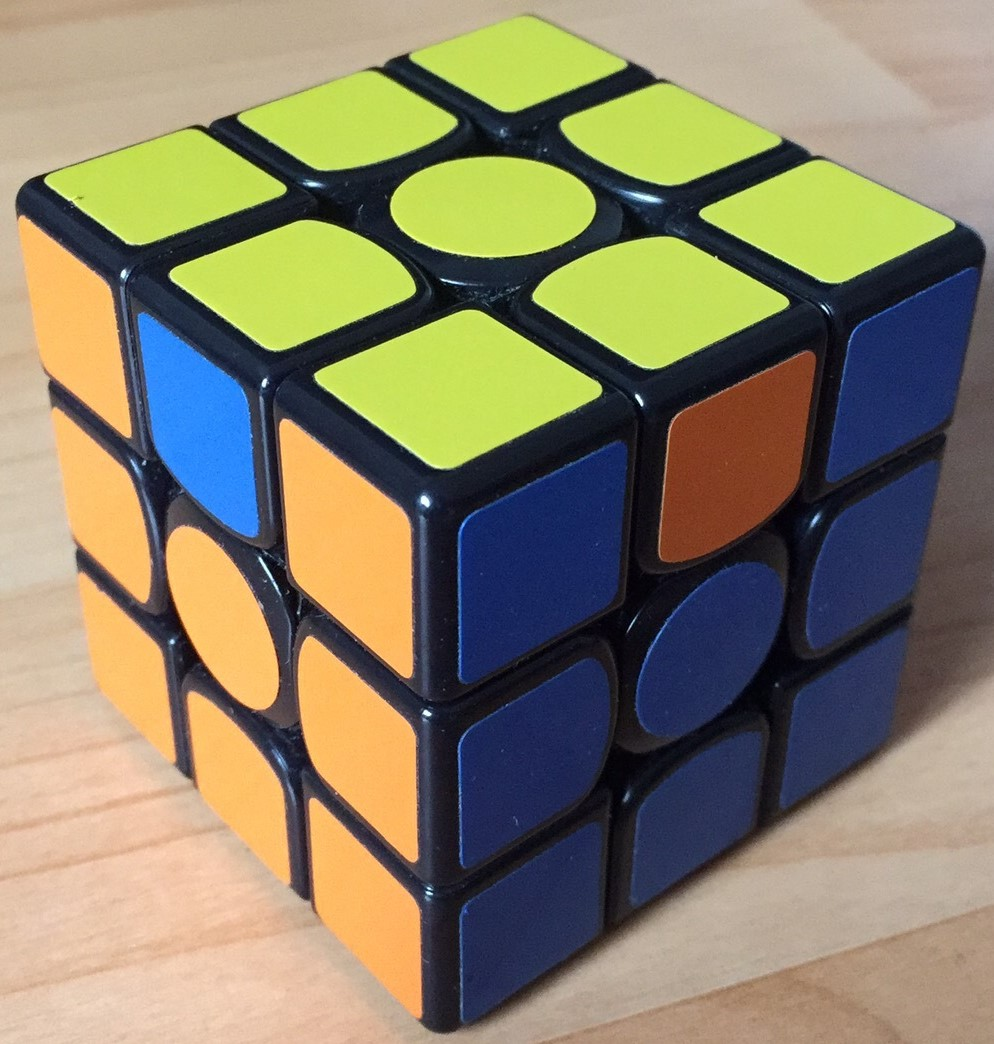
\includegraphics[width=\linewidth]{jh.jpg}
\end{minipage}
\begin{minipage}{0.3\linewidth}
\centering 2.
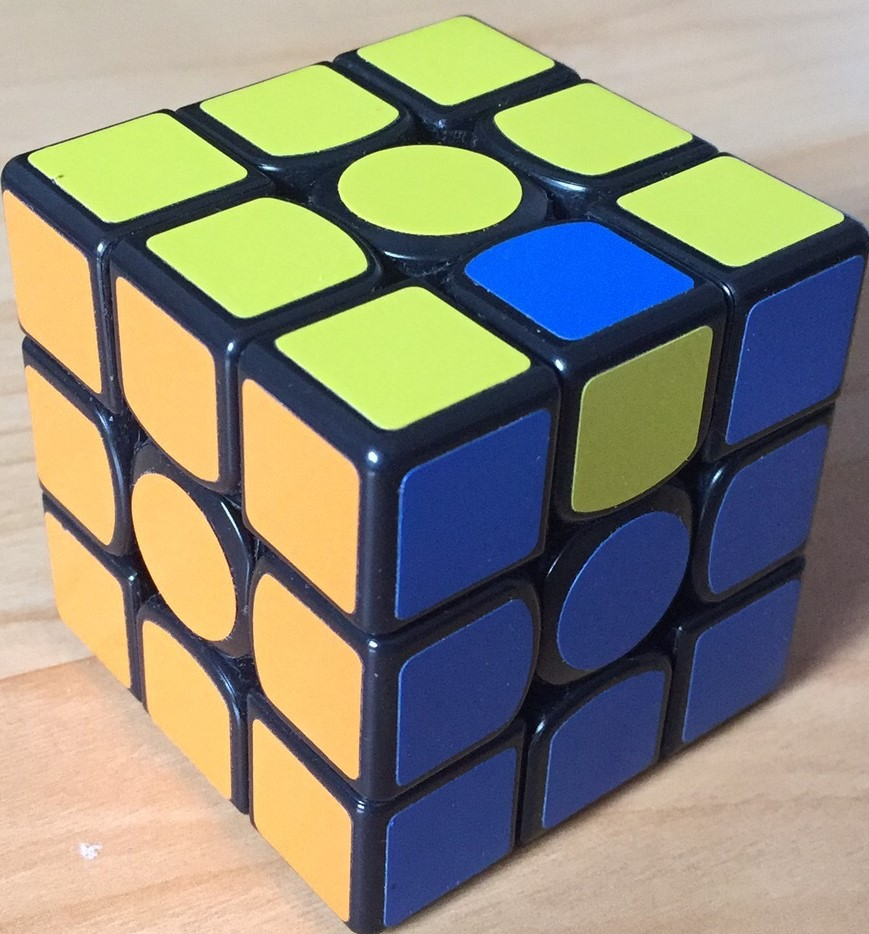
\includegraphics[width=\linewidth]{zl.jpg}
\end{minipage}
\begin{minipage}{0.3\linewidth}
\centering 3.
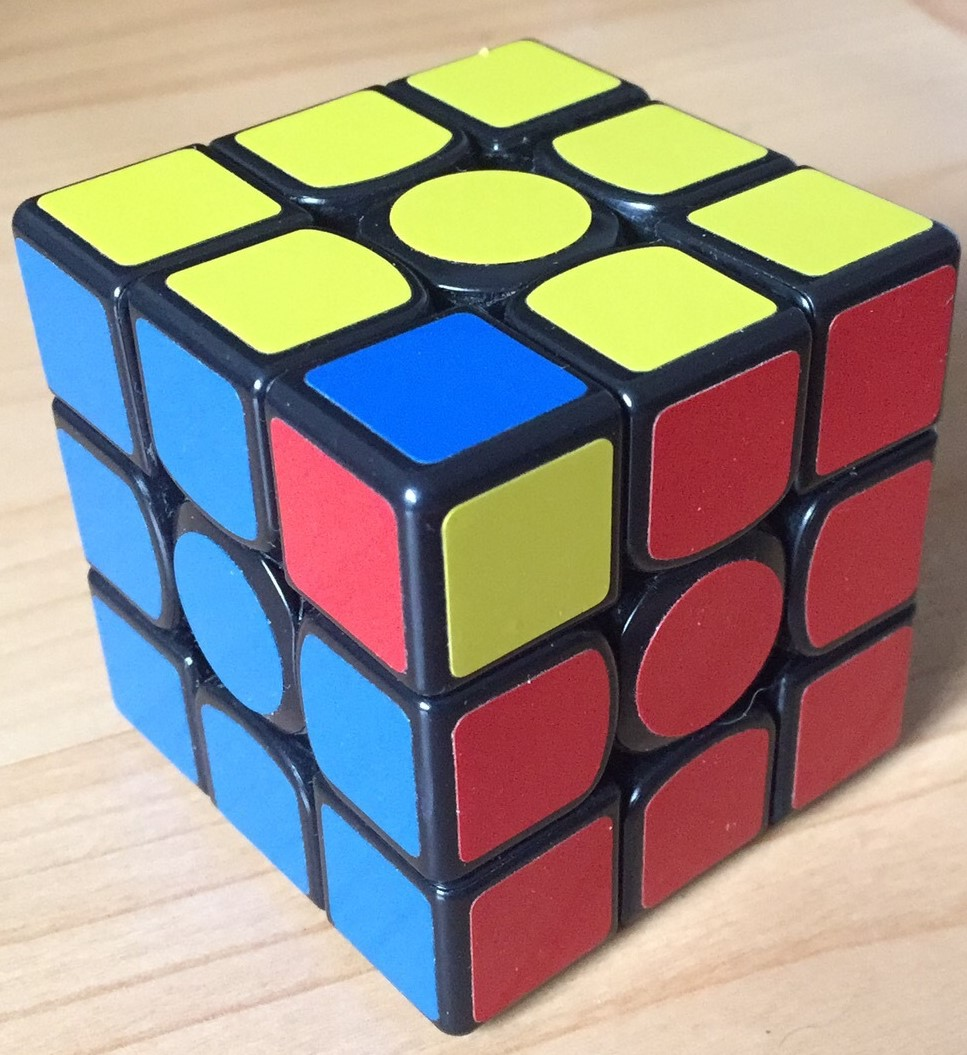
\includegraphics[width=\linewidth]{zj.jpg}
\end{minipage}
(图中看不到的色块都是正确的)
\pr 
(建议配合一个魔方食用)\\
首先我们固定魔方的六个中心(即忽略魔方整体的转动),则魔方的每个操作都由某个面顺时针旋转90度复合构成,我们将对魔方的所有操作组成的集合记作$G$,则$G$关于操作的复合构成一个群。记将黄、白、红、橙、蓝、绿色中心块顺时针转90度为$y,w,r,o,b,g$,称它们为基本操作。则$G=\langle y,w,r,o,b,g\rangle$。记$G$的单位元为$e$,则一个状态$a$可复原当且仅当能通过$G$中的某个元素$a'$对复原状态进行操作能得到状态$a$,易知$a$与$a'$是一一对应的,故以下我们不再区分状态和操作,认为$a$和$a'$是同一对象。
\begin{enumerate}
\item 将魔方的8个角和12个棱编号$1\sim20$,作一个群同态$f:G\To S_{20},f(x)$为$x$对应的状态棱块和角块的置换,易知$f$为一个群同态。且对于每个基本操作$x$,都有$f(x)$为偶置换(因为对应面的棱和角分别构成一个4-循环,故为偶置换),从而$\forall x\in G,f(x)$为偶置换。但图片中的魔方只交换了两个棱块,对应的置换为奇置换,故无法还原。
\item 将魔方的12个棱块的24个色块编号$1\sim 24$,作一个群同态$g:G\To S_{24},g(x)$为$x$对应的状态这些色块的置换(注意即使色块颜色相同也被赋予了不同的编号因此要看成不同的)。注意到对于每个基本操作$x$,都有$g(x)$为偶置换(因为对应面的棱的色块分别构成两个4-循环,故为偶置换),从而$\forall x\in G,g(x)$为偶置换。但图片中的魔方只交换了两个色块,对应的置换为奇置换,故无法还原。
\item 将魔方的8个角编号$1\sim 8$,作一个群同态$\phi:G\To S_{8},\phi(x)$为$x$对应的状态角块的置换。将魔方的白色和黄色中心对应的面称为好面,白色和黄色称为好色。作映射$h_i:G\To \Z_3,h_i(x)$为$x$对应的状态编号为$i$的角块顺时针扭转到好色在好面上需要的次数。由于角块扭转3次和不扭转等价,故映射良定义。且有$h_i(ab)=h_i(b)+h_{\phi(b)(i)}(a)$。作映射$h:G\To\Z_3,h(x)=\dsum_{i=1}^8h_i(x),h(ab)=\dsum_{i=1}^8h_i(ab)=\dsum_{i=1}^8h_i(b)+h_{\phi(b)(i)}(a)=h(a)+h(b)$,故$h$为群同态。对于基本操作$s$,若$s=y,w$,$h_i(s)=0$,故$h(s)=0$。若$s=r,o,b,g$,则有四个$i$使得$h_i(s)=0$,有两个$i$使$h_i(s)=1$,有两个$i$使$h_i(s)=-1$故$h(s)=0$。从而$\forall x\in G,h(x)=0$。但显然题目所给状态对应的$h$为$2$,故无法还原。
\end{enumerate}
\end{Ex}

\begin{Ex}[(前置知识:概率论)]
$N:\Om\To\N,\Pb[N=0]<1$为随机变量,独立地投掷一枚未必均匀的硬币$N$次,每次出现正面的概率为$p$,$X,Y$分别表示$N$次中出现正面和反面的次数。求证:\\$X\dl Y\iff \exists \lambda>0 ,N\sim \mathcal{P}(\lambda)$\\
(选自何辉老师作业)
\pr
令$q:=1-p$\\
“$\Leftarrow$”:
$\forall i,j\in \N$
\vspace{-15pt}\begin{align*}
&\Pb[X=i,Y=j]\\
=&\Pb[X=i,N=i+j]\\
=&\Cb{i+j}{i}p^iq^{j}\frac{\lambda ^{i+j}}{(i+j)!}\exp{-\lambda}\\
=&\frac{p^i}{i!}\frac{q^j}{j!}\exp{-\lambda}\\
=&\frac{p^i}{i!}\exp{-\lambda p}\frac{q^j}{j!}\exp{-\lambda  q }
\vspace{-15pt}\end{align*}
故$X\sim \Poi{\lambda p},Y\sim \Poi{\lambda  q },X\dl Y$
“$\Rightarrow$”:
$\forall i,j\in \N$
\vspace{-15pt}\begin{align*}
&\Pb[X=i,Y=j]\\
=&\Pb[X=i,N=i+j]\\
=&\Pbb{X=i}{N=i+j}\Pb[N=i+j]\\
=&\Cb{i+j}{i}p^iq^{j}\Pb[N=i+j]
\vspace{-15pt}\end{align*}
定义$\left\{\begin{array}{l}f(i):=p^{-i}i!\Pb[X=i]\\
g(j):=q^{-j}j!\Pb[Y=j]\end{array}\right.$则由\\$X\dl Y$,有$(i+j)!\Pb[N=i+j]=p^{-i}i!\Pb[X=i]q^{-j}j!\Pb[Y=j]\!=\!f(i)g(j)$\\
从而
\vspace{-15pt}\begin{align*}
&f(i+1)g(j)\\
=&(i+j+1)!\Pb[N=i+j+1]\\
=&f(i)g(j+1)
\vspace{-15pt}\end{align*}
(1)若$\exists i,f(i)g(i)=0$,\\
令$m\colon=\dmin\{i\colon f(i)g(i)=0\}$,\\
则$f(m)g(m)=0,f(m-1)g(m-1)>0$。不妨设$f(m)=0$,则$\Pb[X=m]=0$,则$\dsum_{k=m}^{+\infty}\Pbb{X=m}{N=k}\Pb[N=k]=0$
则$\forall k\geq m,\Pb[N=k]=0$,但
\vspace{-15pt}\begin{align*}
&\Pb[N=2m-2]\\
\geq & \Pb[X=m-1,Y=m-1]\\
=&\Pb[X=m-1]\Pb[Y=m-1]>0,
\vspace{-15pt}\end{align*}
故$2m-2<m,m=1$,从而$N=0\as$矛盾!故$\forall i,f(i)g(i)\neq 0$\\
(2)$\forall i,j \in \N, f(i)\neq 0,g(j)\neq 0$,则\\
$\exists \lambda>0,\frac{f(i+1)}{f(i)}=\frac{g(j+1)}{g(j)}=\lambda$,则$f(i)=f(0)\lambda ^i,g(j)=j(0)\lambda ^j$,则\\
$(i+j)!\Pb[N=i+j]=f(0)g(0)\lambda^{(i+j)}$,则$\Pb[N=i+j]=\frac{\lambda^{(i+j)}}{(i+j)!}f(0)g(0)$,又有$\dsum_{n=0}^{+\infty} \frac{\lambda^{n}}{n!}f(0)g(0)=1$,则$f(0)g(0)=\exp{-\lambda}$,故$\Pb[N=n]=\frac{\lambda^n}{n!}\exp{-\lambda}$,故$N\sim \Poi{\lambda}$
\end{Ex}

\begin{Ex}[前置知识:数学分析3]
请找出满足下列条件的函数和区间。
\begin{enumerate}
\item 两个累次积分存在而不相等的函数.
\item 二重积分存在而两个累次积分都不存在的函数.
\end{enumerate}
(选自汪林的《数学分析中的问题和反例》)
\pr
\begin{enumerate}
\item 设
$$
f(x, y)= \begin{cases}y^{-2}, & 0<x<y<1, \\ -x^{-2}, & 0<y<x<1, \\ 0, & otherwise\end{cases}
$$
对于 $0<y<1$, 有
$$
\int_0^1 f(x, y) d x=\int_0^y \frac{d x}{y^2}-\int_y^1 \frac{d x}{x^2}=1
$$
因而
$
\dint_0^1 d y \int_0^1 f(x, y) d x=1
$\\
同样地, 对于 $0<x<1$, 有
$$
\int_0^1 f(x, y) d y=-\int_0^x \frac{d y}{x^2}+\int_x^1 \frac{d y}{y^2}=-1
$$
因而
$$
\int_0^1 d x \int_0^1 f(x, y) d y=-1
$$
可见
$$
\int_0^1 d x \int_0^1 f(x, y) d y \neq \int_0^1 d y \int_0^1 f(x, y) d x
$$
\item 
设 $x$ 为一有理数, 则将它表作正分母的既约分数后, 分母表示为 $q_x$. 今在正方形 $D=[0,1] \times[0,1]$ 上定义函数 $f$ 如下:\\
$
f(x, y)= \begin{cases}\frac{1}{q_x}+\frac{1}{q_y}, & x,y\in\Q \\ 0, & otherwise\end{cases}
$\\
兹证 $f$ 在 $D$ 上是可积的. 为此, 我们先来证明 $f$ 在 $D$ 中任一无理点处连续, 而在 其余点处间断.
事实上, 设 $\left(x_0, y_0\right)$ 为 $D$ 中的任一无理点, 对于任给的 $\varepsilon>0$, 只有有限个小于或等于 $\frac{2}{\varepsilon}$ 的正整数. 因此, 使得 $\frac{1}{q_x} \geqslant \frac{\varepsilon}{2}, \frac{1}{q_y} \geqslant \frac{\varepsilon}{2}$ 的有理数 $x=\frac{p_x}{q_x}, y=\frac{p_y}{q_y}$ 只有有限个. 于 是, 存在 $x_0$ (注意, $x_0$ 是无理数!) 的 $\delta$-邻域, 使得适合不等式 $\frac{1}{q_x} \geqslant \frac{\varepsilon}{2}$ 的有理数 $x$ 全在 $\delta$-邻域之外. 同样, 由于 $y_0$ 也是无理数, 故存在 $y_0$ 的 $\xi$-邻域, 使得适合不等式 $\frac{1}{q_y} \geqslant \frac{\varepsilon}{2}$ 的有理数 $y$ 全在 $\xi$-邻域之外. 因此, 存在 $\left(x_0, y_0\right)$ 的一个 $\eta$-邻域, 在这个邻域中, 若 $(x, y)$ 为有理点, 则 $\frac{1}{q_x}+\frac{1}{q_y}<\varepsilon$; 若 $(x, y)$ 不是有理点, 则 $f(x, y)=0$; 而在 $\left(x_0, y_0\right)$ 处, $f\left(x_0, y_0\right)=0$. 由此可知, 当点 $(x, y)$ 落在 $\left(x_0, y_0\right)$ 的 $\eta$-邻域时, 就有\\
$
\left|f(x, y)-f\left(x_0, y_0\right)\right|<\varepsilon .
$\\
于是, $f$ 在 $D$ 中无理点上的连续性得以证明.
设 $\left(x_0, y_0\right)$ 为 $D$ 中的任一有理点, 则
$
f\left(x_0, y_0\right)=\frac{1}{q_{x_0}}+\frac{1}{q_{y_0}}=:r>0 
$\\
因为 $\left(x_0, y_0\right)$ 的任一邻域中都含有无理点 $(x, y)$, 在这种点上 $f(x, y)=0$, 所以当取 $\varepsilon(0<\varepsilon<r)$ 时, 就无法使\\
$
\left|f(x, y)-f\left(x_0, y_0\right)\right|<\varepsilon
$\\
成立. 因此, $f$ 在 $D$ 中的有理点上不连续.设 $\left(x_0, y_0\right)$ 为 $D$ 中任一其余的点, 即 $x_0, y_0$ 不全为有理数, 也不全为无理数. 不妨 设 $x_0$ 为有理数而 $y_0$ 为无理数, 此时 $f\left(x_0, y_0\right)=0$. 在 $\left(x_0, y_0\right)$ 的任一 $\delta$-邻域中都有有 理点 $\left(x_0, y\right)$, 在这种点上, 有\\
$
f\left(x_0, y\right)=\frac{1}{q_{x_0}}+\frac{1}{q_y}>\frac{1}{q_{x_0}}>0 .
$
于是, 当取 $0<\varepsilon<\frac{1}{q_{x_0}}$ 时, 就无法使\\
$
\left|f\left(x_0, y_0\right)-f\left(x_0, y\right)\right|<\varepsilon
$
成立. 因此, $f$ 在 $\left(x_0, y_0\right)$ 处不连续.
现设 $I$ 为 $D=[0,1] \times[0,1]$ 中的全体无理点所成之集, 而 $I_1$ 与 $I_2$ 分别为 $x$ 轴上 的区间 $[0,1]$ 与 $y$ 轴上的区间 $[0,1]$ 中的全体无理点, 则有
$
I=I_1 \times I_2 .
$
因 $m(I)=m(I_1)m(I_2)=1$, 故 $m(D \backslash I)=0$, 可见 $f$ 在 $D$ 上的不连续点所成之集其测度为零. 又, $f$ 在 $D$ 上有界. 因此, $f$ 在 $D$ 上是可积的.
最后, 我们证明 $f$ 在 $D$ 上的两个累次积分都不存在, 从而不能把 $f$ 在 $D$ 上的二重 积分化为累次积分来计算.
我们任意固定 $y \in[0,1]$, 当 $y$ 为有理数时, $q_y$ 为一确定的正整数, 且有\\
$
f(x, y)= \begin{cases}\frac{1}{q_x}+\frac{1}{q_y}, & x \text { 为有理数, } \\ 0, & x \text { 为无理数. }\end{cases}
$\\
易见, $\varphi(x)=f(x, y)$ 在 $[0,1]$ 上无处连续, 从而不可积, 也就根本谈不上 $f$ 在 $D$ 上的累次积分. 另一方向同理。
\end{enumerate}
\end{Ex}
\OMOM




%-------从这里开始——————————



%-------这里结束——————



\end{document}